%===========================================================
%== Präambel ===============================================
%===========================================================
\documentclass[
    paper=a4,
    bibtotocnumbered,
    liststotocnumbered,
    oneside,
    12pt,
    listof=totoc,
    toc=chapterentrywithdots,
    listof=entryprefix,
]{scrartcl}

\usepackage[a4paper, left=2.5cm, right=2.5cm, top=1.25cm, bottom=1.25cm, includehead, includefoot]{geometry}


\usepackage{float}
\usepackage[T1]{fontenc}%Encoding
\usepackage[german]{babel}%German-specific commmands
%\usepackage[utf8]{inputenc} %Wird nicht benötigt bei XeLatex
\usepackage{fancyhdr}%% Kopfzeile u. Fußzeile
\usepackage{fontspec}%% Schriftart
\usepackage[onehalfspacing]{setspace}%-- Zeilenabstand 1,5
\usepackage[toc, nopostdot, acronyms]{glossaries}%% Glossar
\usepackage[intoc]{nomencl}%% Symbolverzeichnis
\usepackage{etoolbox}%Sorgt dafür, das Symbolverzeichnis im Header steht
%\usepackage{listings}
\usepackage[]{minted}
\usepackage[titles]{tocloft}
\usepackage{scrhack}
\usepackage{colortbl}%Einfärben von Tabellen-Zellen, Zeilen, Spalten
\usepackage[]{layout}
\usepackage[]{blindtext}
%\usepackage{showframe}% zum Anzeigen des Seitenlayouts
\usepackage[figurename={Abb.},tablename={Tab.}]{caption}%Anpassung der Namen für Abbildung und Tabelle
\usepackage[]{url}
\usepackage[]{hyperref}
\usepackage{chngcntr}%% Nummerierung der Abbildungen und Tabellen fortlaufend %%%%%%
\usepackage{tocbibind}
\usepackage[style=alphabetic, citestyle=alphabetic]{biblatex}
\usepackage[babel,german=quotes]{csquotes} % Deutsche

% Paragraph styles
\setlength{\parindent}{0cm}
\setlength{\parskip}{6pt}

%% Kopfzeile u. Fußzeile
\pagestyle{fancy}
\fancyfoot{}
\fancyfoot[R]{\thepage}
\fancyhead{}
\fancyhead[L]{\nouppercase{\leftmark}}
\fancypagestyle{plain}{\pagestyle{fancy}}

%-- Standardschriftart auf Times New Roman umstellen
\setmainfont[ Path = Fonts/,
BoldFont=timesbd.ttf,
ItalicFont=timesi.ttf,
BoldItalicFont=timesbi.ttf
]{times.ttf}

%-- Kapitelüberschriften auf Standardschriftart(Times New Roman) umstellen
\setkomafont{disposition}{\normalcolor\bfseries}

% Entfernt "Kapitel X" aus der Kopfzeile vor der Kapitelüberschrift
%\renewcommand{\chaptermark}[1]{\markboth{\MakeUppercase{#1}}{}}
 
% %Abstände nach Kapiteln 
% \RedeclareSectionCommand[%
%   beforeskip=0pt,
%   afterskip=1\baselineskip plus .1\baselineskip minus .167\baselineskip
% ]{chapter}

%% Nummerierung der Abbildungen und Tabellen fortlaufend %%%%%%
\counterwithout{figure}{section}
\counterwithout{table}{section}

%% Rahmen in Textbreite um Bilder
\floatstyle{boxed}
\restylefloat{figure}
\restylefloat{table}
\restylefloat{listing}

%% Captions linksbündig orientieren
\captionsetup{justification=raggedright,singlelinecheck=false}

% Einbinden von Glossar u. Abkürzungsverzeichnis
%-----------------------------------------------------------------------------
% Glossar
%-----------------------------------------------------------------------------

\newglossaryentry{computer}
{
    name=computer,
    description={is a programmable machine that receives input,
    stores and manipulates data, and provides
    output in a useful format}
}
\input{Verzeichnisse/Abkürzungsverzeichnis.tex}
% \makeglossaries

\renewcommand{\labelenumi}{\arabic{enumi}.} 
\renewcommand{\labelenumii}{\arabic{enumi}.\arabic{enumii}}
\renewcommand{\labelenumiii}{\arabic{enumi}.\arabic{enumii}.\arabic{enumiii}}

\usepackage{enumitem}
\setlist[2]{nosep}
%\setlist[1]{nosep}

\addbibresource{Literatur/literatur.bib}
\addbibresource{Literatur/internet.bib}
\addbibresource{mendeley.bib}
\DeclareFieldFormat{formaturl}{\newline #1}
\renewbibmacro*{url+urldate}{%
\printtext[formaturl]{%
  \printfield{url}}%
  \iffieldundef{urlyear}
    {}
    {\setunit*{\addspace}%
     \printtext[]{\printurldate}}}

\begin{document}

%===========================================================
%== Titelseite =============================================
%===========================================================
\newgeometry{left=2.5cm, right=2.5cm, top=2.5cm, bottom=2.5cm}
\begin{titlepage}
    \begin{center}
    
\includegraphics[width=\textwidth]{Images/logo}
        \begin{Large}
        Hochschule für angewandte Wissenschaften Coburg
        \\
        Fakultät Elektrotechnik und Informatik
        \par
        \end{Large}
        \vspace{2.0cm}
        
        \begin{Large}
            Studiengang: Informatik
            \par
        \end{Large}
        \vspace{1.5cm}
        
        \begin{Large}
            Exposé zur Bachelorarbeit
        \end{Large}
        \vspace{2.0cm}

        \begin{huge}
            \textbf{- Titel der eigenen Arbeit, eine oder maximal drei Zeilen -} 
            \par
        \end{huge}        
        \vfill
        
        \begin{huge}
            Daniel Müller
        \end{huge}
        \vspace{2.0cm}
        
        \begin{large}
            %Abgabe der Arbeit: DD. Monat 2015
            
            Betreut durch:
            \\
            <Prof. Dr.> <Vorname> <Nachname>, Hochschule Coburg
            \\
            %<optional: Zweitgutachter: Prof. Dr. XXX, Hochschule Coburg>
            \par
        \end{large}
        
    \end{center}
\end{titlepage}
\restoregeometry
    
%===========================================================
%== Inhaltsverzeichnis =====================================
%===========================================================   
\begin{singlespace}
\renewcommand{\cftsecleader}{\cftdotfill{\cftdotsep}} % Punkte im Inhaltsverzeichnis bei Kapiteln
\tableofcontents
\end{singlespace}
\newpage

% %===========================================================
% %== Abbildungsverzeichnis ==================================
% %===========================================================
% \newpage
% \renewcommand{\cftfigpresnum}{Abb. }
% \renewcommand{\cftfigaftersnum}{:}
% \setlength{\cftfignumwidth}{2cm}
% \setlength{\cftfigindent}{0cm}
% \listoffigures

% %===========================================================
% %== Tabellenverzeichnis ====================================
% %===========================================================
% \newpage
% \renewcommand{\cfttabpresnum}{Tab. }
% \renewcommand{\cfttabaftersnum}{:}
% \setlength{\cfttabnumwidth}{2cm}
% \setlength{\cfttabindent}{0cm}
% \listoftables

% %===========================================================
% %== Codeverzeichnis ========================================
% %===========================================================
% \newpage
% \renewcommand\listingscaption{Code}
% \renewcommand\listoflistingscaption{Codebeispielverzeichnis}
% \renewcommand{\cftfigpresnum}{Code }
% \listoflistings
% \addcontentsline{toc}{chapter}{Codebeispielverzeichnis}

% %===========================================================
% %== Symbolverzeichnis ======================================
% %===========================================================
% \newpage
% %% Symbolverzeichnis
% \makenomenclature
% % This will add the units
% %----------------------------------------------
% \newcommand{\nomunit}[1]{%
% \renewcommand{\nomentryend}{\hspace*{\fill}#1}}
% %----------------------------------------------
% \renewcommand{\nomname}{Symbolverzeichnis}
% %Sorgt dafür, das Symbolverzeichnis im Header steht
% \patchcmd{\thenomenclature}
%   {\chapter*{\nomname}}% usually only \chapter*{\nomname} is issued
%   {\chapter*{\nomname}\markboth{\MakeUppercase\nomname}{\MakeUppercase\nomname}}
%   {}{}
% %-----------------------------------------------------------------------------------
% Symbolverzeichnis
%-----------------------------------------------------------------------------------
% Bsp: \nomenclature[prefix]{symbol}{description}

\nomenclature[]{$c$}{Speed of light in a vacuum inertial system \nomunit{$299,792,458\, m/s$}}

\nomenclature[]{$i$}{Ganzzahlige Laufvariable \nomunit{Integer}}
% \printnomenclature


% %===========================================================
% %== Abkürzungsverzeichnis ==================================
% %===========================================================
% \newpage
% \printglossary[type=\acronymtype, title=Abkürzungsverzeichnis, toctitle=Abkürzungsverzeichnis]
%<<<<<<<<<<<<<<<<<<<<<<<<<<<<<<<<<<<<<<<<<<<<<<<<<<<<<<<<<<<<<<<<<<<<<<<<<<<<<<<<<<<<
% Text Einleitung, Hauptteil usw. 
%<<<<<<<<<<<<<<<<<<<<<<<<<<<<<<<<<<<<<<<<<<<<<<<<<<<<<<<<<<<<<<<<<<<<<<<<<<<<<<<<<<<<

\section{Motivation und Problemstellung}
Neben den etablierten Programmiersprachen wie Java, C/C++ werden kontinuierlich neue Programmiersprachen entwickelt. 
Unter den Top5 der mit GitHub verwalteten Programmiersprachen befinden sich mit Swift von Apple und Go von Google zwei Projekte die von bedeutenden IT-Firmen stammen. (siehe Abbildung\ref{figure:github})

	\begin{figure}[h]
	\centering
	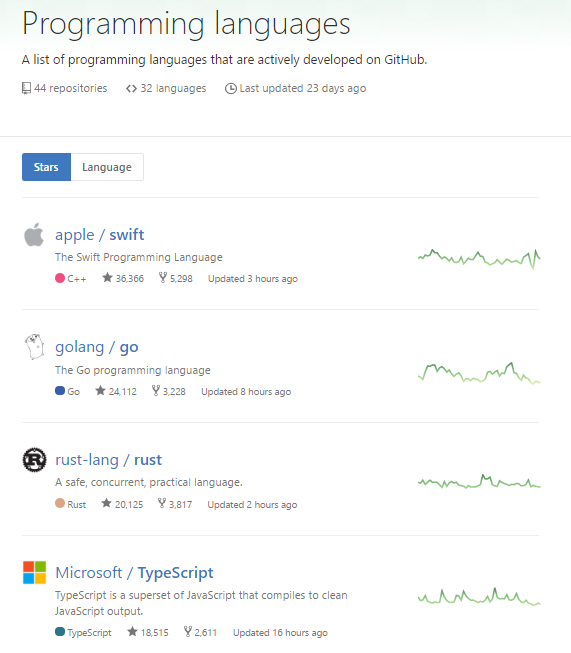
\includegraphics[width=0.5\textwidth]{Images/github}
	\caption{Ranking der unter GitHub verwalteten Programmiersprachen Stand: 26.01.2017 Quelle: Github.com}%
	\label{figure:github}%
	\end{figure}

Doch warum bedarf es der Entwicklung neuer Programmiersprachen?
\begin{quote}
\enquote{Google wollte sich nicht damit zufriedengeben, das die Unterstützung aktueller Trends in der Systemsoftwareentwicklung wie Parallelisierung, Cloud-Computing etc. in den etablierten Hochsprachen nur mehr schlecht als recht ergänzt wurde.} \cite{Feike2011}
\end{quote}

Was macht Swift interessant?
\begin{quote} 
\enquote{Interessanterweise ist ein nicht unwesentlicher Punkt bei der Beantwortung dieser Frage die bisherige Sprache der Apple-Plattform: Objective-C.} \cite{Popp.2015}
\end{quote}

\section{Forschungsfrage}
Im Rahmen dieser Bachelorarbeit soll Swift und Go anhand von definierten Kriterien verglichen werden. Hierbei stellen sich folgende Kernfragen:

\begin{samepage}
\begin{itemize}
    \item Ist objektorientierte Programmierung möglich? 
    \item Kann funktionale Programmierung eingesetzt werden?
    \item Welche Möglichkeiten werden zur Nebenläufigen Programmierung geboten?
    \item Kann im konkreten Fall eine Webanwendung implementiert werden? Welche Komponenten/Frameworks werden dafür eventuell benötigt?
\end{itemize}
\end{samepage}

In den Punkten objektorientierte Programmierung und funktionale Programmierung stellt sich die Frage, wie sich Swift und Go zu den bereits etablierten Programmiersprachen unterscheiden beziehungsweise ähneln. 
Was machen Swift und Go anders als die etablierten Programmiersprachen?

\section{Methode}
Swift und Go sollen anhand folgender Kriterien verglichen werden:

\begin{itemize}%[nosep]
    \item \textbf{Syntax}
    \begin{itemize}
        \item Funktionen (Definition und Aufruf)
        \item Variablen (Deklaration und Definition)
        \item Kontrollstrukturen
        \item Blockstrukturen
        \item Operatoren
    \end{itemize}
    \item \textbf{Typsystem}
    \begin{itemize}
        \item Wie werden Null-Werte behandelt?
        \item Welche Art von Typisierung?
        \item Typinferenz möglich?
        \item Referenz- und Wertegleichheit
    \end{itemize}
    \item \textbf{Fehlerbehandlung}
    \begin{itemize}
        \item Welche Möglichkeit zur Fehlerbehandlung gibt es?
        \item Gibt es Exceptions?
    \end{itemize}
    \item \textbf{Speicherverwaltung}
    \begin{itemize}
        \item Garbage Collection
    \end{itemize}
    \begin{samepage}
    \item \textbf{Generische Programmierung}
    \begin{itemize}
        \item Gibt es Generics?
    \end{itemize}
    \end{samepage}
    \item \textbf{Nebenläufigkeit}
    \begin{itemize}
      \item Welche Möglichkeiten gibt es zur nebenläufigen Programmierung?  
    \end{itemize}
    \item \textbf{Objektorientierte Programmierung}
    \begin{itemize}
        \item Datenkapselung
        \item Abstraktion
        \item Vererbung, evtl. Mehrfachvererbung
        \item Polymorphismus
    \end{itemize}
    \item \textbf{Funktionale Programmierung}
    \begin{itemize}
      \item First-Class Funktionen
      \item High-Order Funktionen
      \item Referenzielle Integrität
      \item Closures/Lambda-Ausdrücke
    \end{itemize}
  \item \textbf{Anwendungsbeispiel: Webanwendung}
  \begin{itemize}
    \item Benötigte Frameworks
  \end{itemize}
  \item \textbf{Tools/Werkzeuge}
  \begin{itemize}
    \item Gibt es bereits IDE's?
    \item Frameworks für Softwaretests
  \end{itemize}
\end{itemize}

Soweit möglich, soll jedes Kriterium anhand eines aussagekräftigen Beispiels veranschaulicht werden.
Die Gewichtung der Vergleichskriterien sind in Abbildung \ref{figure:gewichtung} zu sehen.

	\begin{figure}[h]
	\centering
	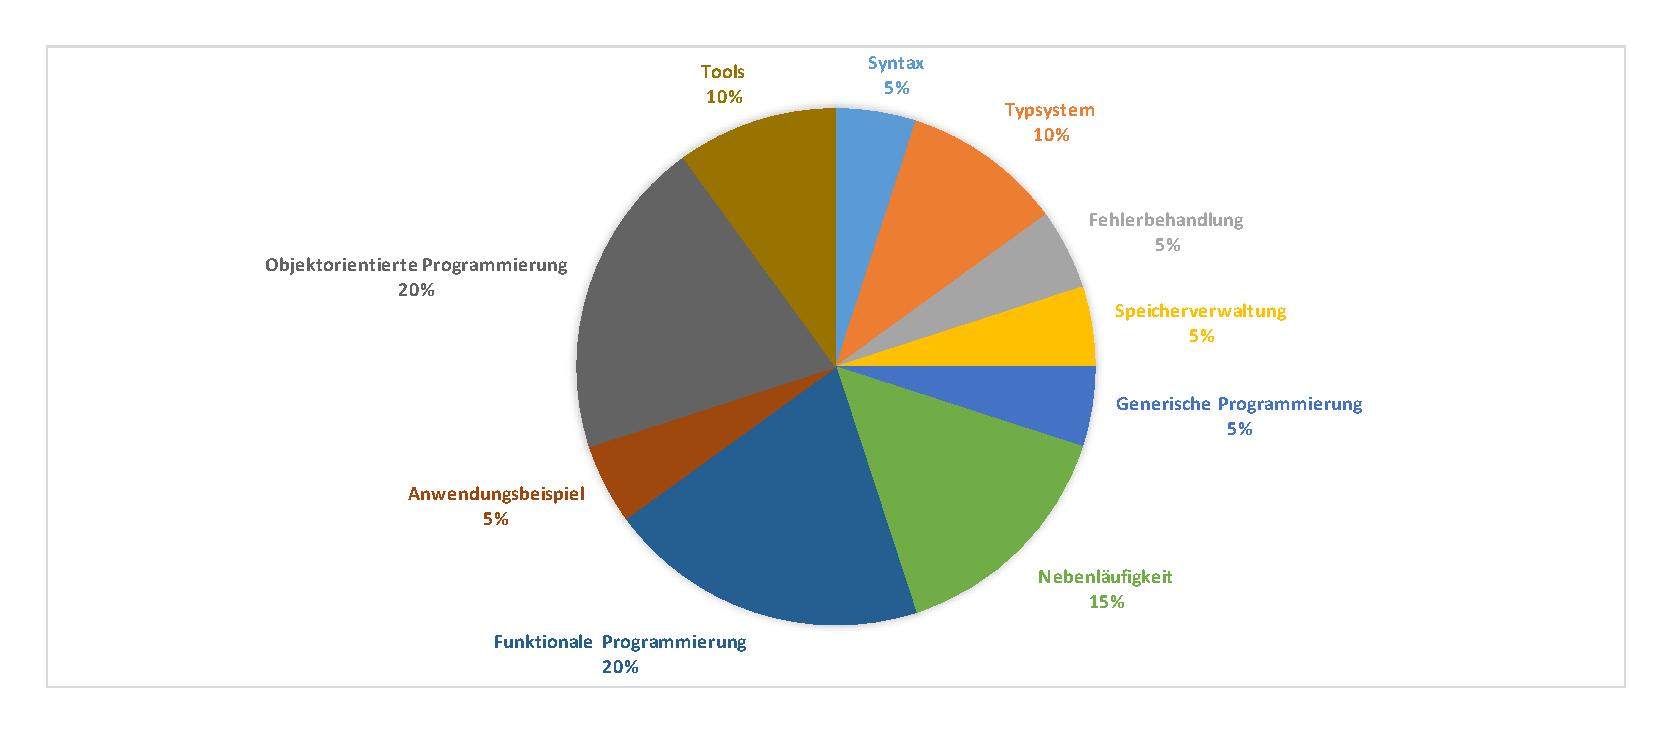
\includegraphics[width=0.6\textwidth]{Images/gewichtung}
	\caption{Gewichtung der Vergleichskriterien}%
	\label{figure:gewichtung}%
	\end{figure}

\section{Gliederung}

\begin{samepage}
\begin{enumerate}
    \item \textbf{Einleitung}
    \begin{enumerate}
        \item Kontext der Arbeit
        \item Zielsetzung/Motivation
        \item Aufgabenstellung
        \item Aufbau der Arbeit
    \end{enumerate}
    \item \textbf{Syntax}
    \item \textbf{Typsystem}
    \item \textbf{Fehlerbehandlung}
    \item \textbf{Speicherverwaltung}
    \item \textbf{Generische Programmierung}
    \item \textbf{Nebenläufigkeit}
    \item \textbf{Objektorientierte Programmierung}
    \item \textbf{Funktionale Programmierung}
    \item \textbf{Anwendungsbeispiel: Webanwendung}
    \item \textbf{Tools}
    \item \textbf{Zusammenfassung}
    \item \textbf{Ausblick}
\end{enumerate}
\end{samepage}
\newpage

\section{Zeitplan}

\begin{table}[h]
\centering
\begin{tabular}{|c|c|} 
 \hline
 \rowcolor[gray]{0.75} \textbf{Zeitraum} & \textbf{Aufgabe} \\
 \hline
 Februar 2017 & Syntax, Typsystem, Fehlerbehandlung... \\ 
 \hline 
 März 2017 & Objektorientierte Programmierung, Funktionale Programmierung \\
 \hline 
 April 2017 & Generische Programmierung, Nebenläufigkeit, Speichervewaltung \\
 \hline
 Mai 2017 & Anwendungsbeispiel, Tools, Einleitung u. Zusammenfassung \\
 \hline
\end{tabular}
\caption{Zeitplan}
\label{table:zeitplan}
\end{table}

% %===========================================================
% %== Glossar ================================================
% %===========================================================
% %% Glossar
% \renewcommand*{\glossaryentrynumbers}[1]{} %Entfernt die Seitenzahl am Ende der Glossar-Beschreibung

% \printglossary[title=Glossar,toctitle=Glossar]

%===========================================================
%== Literaturverzeichnis ===================================
%===========================================================
\newpage
\nocite{*}
% \bibliography{Literatur/literatur.bib,Literatur/test.bib,mendeley.bib}
% \bibliographystyle{alphadin}

\printbibliography[heading=bibintoc,title={Literaturverzeichnis}]

%===========================================================
%== Anhang =================================================
%===========================================================
% \appendix
% \chapter{Anhang}
% \newpage
% \section{Ehrenwörtliche Erklärung}
% \begin{centering}
\textbf{{\huge Ehrenwörtliche Erklärung}}
\par
\end{centering}

\vspace{2cm}

Ich versichere hiermit, dass ich meine/n Praxisbericht/Bachelorarbeit/Masterarbeit mit dem Titel

\vspace{2cm}

\begin{tabular*}{\linewidth}{@{\extracolsep{\fill}}ccc}
 \\ \hline
 \vspace{2cm}
 \\ \hline
\end{tabular*}

\vspace{2cm}

selbständig verfasst, keine anderen als die angegebenen Quellen und Hilfsmittel benutzt sowie nicht an anderer Stelle als Prüfungsarbeit vorgelegt habe.

\vfill

\begin{tabular}{ccc}
\cline{1-1}
\parbox{7cm}{\raggedright Ort} &
\parbox{3cm}{\raggedright} &
\parbox{7cm}{\raggedright} \\
\vspace{2.5cm} \\
\cline{1-1} \cline{3-3}
\parbox{7cm}{\raggedright Datum} &
\parbox{3cm}{\raggedright} &
\parbox{7cm}{\raggedright Unterschrift} \\ 
\end{tabular}

\end{document}
